\chapter{Implementation} \label{chapter:implementation}
This chapter explores the development phase of the simulator following the outlined design structure. The implementation of the project took place in iterations in order to prioritize features and to decrease the overall complexity of implementing all the requirements at once. The complete source code can be found in Appendix \ref{appendix:code}. Appendix \ref{appendix:userGuide} explains how to use the simulation tool, and Appending \ref{appendix:setupguide} explains how to run the code locally.


\section{Introducing used Technologies}
This section is an overview of the technologies implemented during the project so as to give a brief introduction of which library or framework has been employed for each part of the architecture.


\subsection{Node.js \& Express.js}
Node.js is JavaScript run-time environment to create servers. It supports useful features such as asynchronous Input/Output, and real-time communication. The community of this language offers the largest collection of open source libraries in the world. It has been chosen for the simulator because it is specifically designed to create web applications and it has modules for real-time communication and cryptography functions that are the main functionalities needed for the simulation. In addition, it unifies the application with a single main programming language as JavaScript is used both for back-end and front-end development \cite{Nodejs}. 

Express.js is lightweight framework that helps to build a web application and server static files and resources through a simple-to-use API. For the purpose of this project, node.js would suffice. However, express.js is employed to write less manual/verbose commands that node.js would require.

\subsection{Socket.io}
Socket.io is a real-time library for bi-directional communication between clients and servers. The availability of this library only in JavaScript was one of the main reasons to choose Node.js as the preferred server-side environment. This library is based on web sockets, a communication protocol, and it serves as a high-level wrapper to them.

The communication is event-based. Therefore, the some action needs to happen in order to trigger the execution of some code usually stored in an 'event handler' function.
The ease of use of this library makes it easy to create a real-time applications allowing the effort of development to be focused on the security properties that the simulation needs to achieve, rather than being slowed down by how to create a distributed system and exchange messages with low latency.

The library can be used both on the back-end and front-end, so a client and a server can use the same functions (from the API) to trigger or handle events.


\subsection{React.js}
This is another JavaScript library that allows modular development of graphical user interfaces (GUI) in the form of 'components' that can be reused. It is a uncomplicated to create an interface that are interactive and change aspect based on the state of the application.

Therefore, it is a very handy library to create this simulation tool, to create a self-explanatory GUI that will be updated at each stage of the protocol execution.

React.js is used in conjunction with JSX, a special syntax to describe what the UI should look like based on the logic state of the application/component, which is a mixture of HTML and JavaScript.

Since JSX is a special syntax that needs to be 'transpiled' into plain JavaScript and HTML that the browser can understand. In order to do, 'Babel' transpiler will be used through in conjunction with a module bundler technology called 'Webpack'. This latter simply merge together several components created during the development phase into a unique 'bundle' file that will be sent to the browser.

Indeed, the set up for this library is not straightforward, but it is a valuable asset in building a state-based UI.

\subsection{Other third-parties Libraries}
The following are other libraries utilized for significant functionalities of the system that helped both in terms of functionalities and sped up the development phase.

\subsubsection{Cryptographically Secure Pseudo-Random Number Generator (csprng)} \label{sec:csprng}
A pivotal code functionality to be implemented successfully is a random generator that produces cryptographically secure numbers to be used as secret keys for each adjacency. A generator that provides this property means that each number is equally likely to be generated, preventing any sort of attack based on the statistical frequency of a stream of generated numbers. 
For this reason, the 'random-number-csprng' library has been implemented, where possible, instead of writing functions that manually generate a random number in a given range.

\subsubsection{Random Name Generator}
The final application will support an arbitrary number of participants connected to the application. In order to identify them among each other a Node library to generate random names has been implemented called 'node-random-name'. 

\subsubsection{Mocha \& Chai} \label{sec:testingFrameworks}
An important aspect for a mature application is to employ a framework for unit-testing, which is a method to prove the correctness of the logic of an application by verifying the output of a unit being tested is indeed what was expected.

In order to do so in this application, the testing frameworks used is Mocha in conjunction with the assertion library Chai. 


\section{Development Approach}
The approach used throughout the project is a lean methodology that consists in brief iterations of design, implementation and testing. This allowed flexibility to review direction and aims of the initial proposal during project evolution. In addition, making use of iterations helped to be mindful of the time and resource constraints that, as in any other project, were present. Namely, iterations assisted the prioritization of which aspects were more important and what were the dependencies between features to arrange their execution sensibly. This approach lead to the division of the requirements in basic and advanced.


The implementation of functionalities progressed in the following order:
\begin{enumerate}
    \item Implement hard-coded version of the protocol in a single JavaScript file with three participants represented by variables and using a general number random generator;
    \item Develop Node.js web application integrated with React.js and transpiling pipeline of Webpack and Babel;
    \item Integrate Socket.io with React.js for real-time communication;
    \item Distribute the execution of basic protocol between clients and server. Each client possess logic functions inside the main React component (AppComponent). The server generates adjacencies and reacts to events such as connection and disconnection of a client which may trigger the start of the protocol;
    \item Substitute simple random generator with a cryptographically secure pseudo-random number generator;
    \item Implement random name generator to have unique client names;
    \item Introduce objects (Adjacency, Participant, Round) to group functionalities and attributes together and improve modularity of the codebase;
    \item Implement security mechanism to abort communication with less than 3 clients;
    \item Implement clean-up functionalities for the client's browser. This clears keys and other local data when communication is aborted but then restarts again;
    \item Refactor code after having implemented all of the basic features, separating, where possible, the logic of the protocol from the sever-client communication functions;
    \item Implement helper messages on hover for the main steps of the protocol execution;
    \item Start Unit-Testing of the logic functions;
    \item Refactor the AppComponent into smaller React components, each responsible for a single element of the GUI;
    \item deploy application 
    \item Repeat protocol execution continuously, so as to have multiple rounds of communication;
    \item Support connection of an arbitrary number of clients to the server;
    \item Handle connection and disconnection of clients in the middle of round execution;
    \item Implement key storage on the server and utilize this to detect collision;
    \item Implement 8-bit keys;
    \item Divide communication into three types of rounds (voting round, length-calculation round, communication round) and all the relative features that this division entails;
    \item Implement the new security mechanisms needed: prevent the message sender to win the next voting round; abort round when message sender disconnects during round; abort communication if all clients try to send a message in the same round;
    \item Refine user-interface to improve user-friendliness and perform final refactor of codebase;
\end{enumerate}


\subsection{Development Pipeline Tools}
To publish the simulator online, a continuous integration development pipeline was created. This simply means that new features are available live as soon as the codebase updates happen, ensuring that the application is tested correctly. \newline

Firstly, the code is uploaded on Github, a code-sharing platform where a user can store projects.

Secondly, through the presence of a webhook on Github, a code update will trigger the automatic execution of unit-tests in Circle CI (continuous integration). This ensures that new features did not break functionalities previously built.

Lastly, If all tests successful the code is automatically released on the web hosting platform Heroku. The application is in fact available at \url{https://www.dc-net.herokuapp.com}.

\begin{figure}[h!]
    \centering
    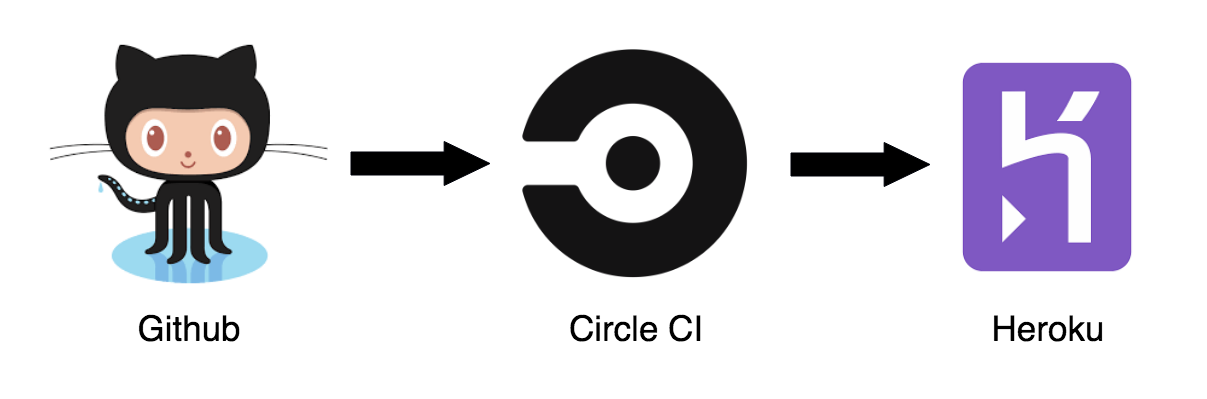
\includegraphics[width=0.70\textwidth]{Images/pipeline.png}
    \caption{Development Pipeline}
    \label{fig:devPipeline}
\end{figure}

\section{Basic Implemented System}
This section presents the main components of the simulator implemented at the completion of the basic requirements. 

\emph{Please note that all the features presented are implemented in the code. However, some of the code snippets presented in this section are not exactly the same as in the source code, since the version provided in the appendix is the final product that also includes the advanced requirements.}

\subsection{Initial Connection} \label{sec:initialConnection}
A client that connects to the server, by typing \lstinline{https://www.dc-net.herokuapp.com} in his browser, will automatically trigger a socket \lstinline{connection} event. This turns the simple \lstinline{HTTP get} request of the page into a \lstinline{TCP} session. This happens thanks to a \lstinline{HTTP Upgrade} request. The result is a stable open connection between a client and a server, and both ends listen to incoming \lstinline{socket.io} events.


\subsection{Socket.io communication example}
\lstinline{Socket.io} provides an API that is used by the server to trigger, i.e. emit, real-time events that will instantly reach the client/clients (figure \ref{fig:incomingConnection}). 

\begin{figure}[H]
    \centering
    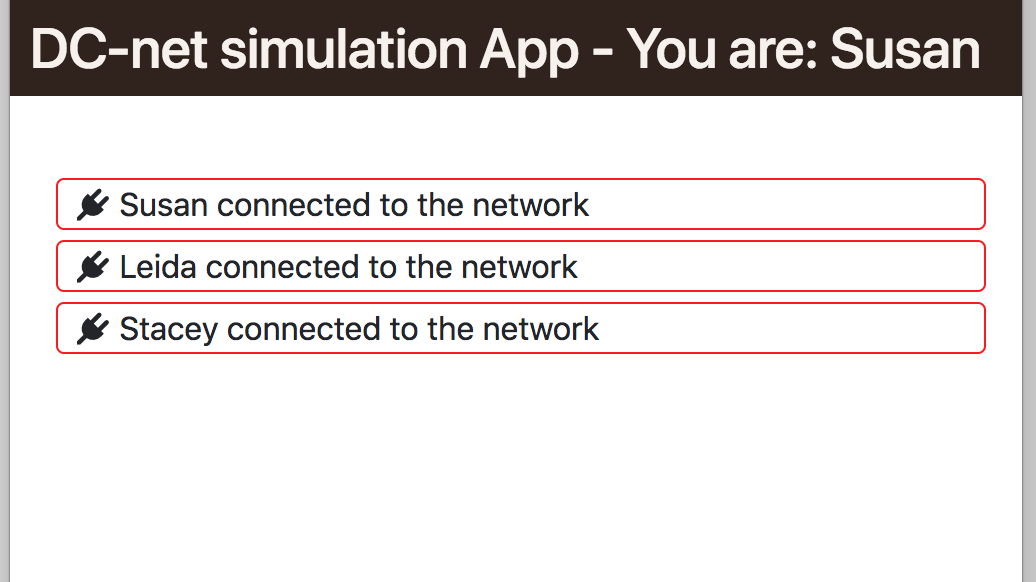
\includegraphics[width=0.5\textwidth]{Images/Implementation/incomingConnections.png}
    \caption{Incoming connections displayed on a client}
    \label{fig:incomingConnection}
\end{figure}

The following are two examples of \lstinline{emit} events: 
\begin{lstlisting}
  /* server sends broadcast event 'client-connection' to all connected clients and sends them the name of the participant that just connected*/
  io.sockets.emit('client-connection', newParticipant.name);
  
  /* server sends unicast event 'client-connection' to client1 with the name of the name of the participant that just connected */
  io.sockets.to(client1.id).emit('client-connection', newParticipant.name);
\end{lstlisting}

The first parameter of the emit function is always the event name, and the optional following parameters are the data being sent. \newline

In order for a client to handle an event emitted by the server the function \lstinline{socket.on('event-name')} is employed. A small API to combine React.js and Socket.io was created (source code file \lstinline{socket-api.js}). Each function developed is a wrapper function that receives a callback as a parameter to be invoked when the specific socket event is received by the sever. For Example: 
\begin{lstlisting}
    // example of wrapper function to socket.on event.
    function connectionEvent(callback) {
        /* client socket listens to 'client-connection' event. When receiving this event a single paramenter 'name' is expected */
        socket.on('client-connection', (name) => {
                // invoking function that was passed as a parameter
                callback(name);
            }
        );
    }
\end{lstlisting}

The client provides the callback parameter for a socket event in the React.js component called \lstinline{AppComponent}. In fact, only the \lstinline{AppComponent} in the developed application will interact with socket events, so that there exist a centralized place to communicate with the back-end. The \lstinline{socket-api.js} functions are imported in the \lstinline{AppComponent} and, following the example above, the callback to the \lstinline{connectionEvent} function can be provided as follows: 
\begin{lstlisting}
    /* connectionEvent function called with an arrow function as parameter, which is the callback that will be invoked when the socket event 'client-connection' will be received */
    connectionEvent((name) => {
        /* update state of AppComponent adding a connection object to the list of events */
        this.setState({
            events: [...this.state.events, new Connection(name)],
        });
    });
\end{lstlisting}

In the same way, a client can emit an event with \lstinline{socket.emit('event-name1');} and this will be received by the server. If the this latter has a corresponding \lstinline|socket.on('event-name1', () => { /* do something on the server */  });| then, an action is triggered. \newline


To summarize, all the exchanges between the server and the client, with exception of the initial \lstinline{HTTP get} request, will take place through \lstinline{socket.io} real-time library. Both the server and clients can emit and listen to events, and perform some computation accordingly. 


\subsection{State of Client \& UI updates}
React.js front-end components can have their own state. This is simply an object where information of that component is stored.
\begin{lstlisting}
    // state object example of basic implementation. A state can be intialized in the constructor of the React component.
    this.state = {
        events: [],
        showDiagol: false,
        roundNumber: 0,
        roundInProgress: false,
        whoami: '',
    };
    
    // example command to access the roundNumber variable of the state
    this.state.roundNumber;
    
    /* how to update state. Need to use setState() function cannot change state variables directly */
    this.setState({
        roundNumber: ++roundNumber;
    });
\end{lstlisting}

The React.js feature that updates the user interface is the automatic re-rendering triggered when \lstinline{this.setState()} function is invoked.

This is a simple yet powerful concept that allows a granular manipulation of the interface.


\subsection{Trigger execution of the protocol} \label{sec:triggerProtocol}
The server starts of the execution of the protocol as soon as three clients establish a connection. This is possible because, as mentioned in section \ref{sec:initialConnection}, a \lstinline{connection} event is emitted by the client at connection time and received by the server. The basic version of the connectionHandler on the server creates a new Participant objects and stores it in a list to keep track of the current connections, it broadcasts to all clients the fact that a new connection happened, and if at least three users are connected the protocol begins.

\begin{lstlisting}
    // handle a new client connection on connection on the server.
    function handleNewConnection(socket) {
        var newParticipant = new Participant(generateUniqueRandomName(participants), socket.id);
        participants = [...participants, newParticipant];
        broadcastEvent('client-connection', newParticipant.name);
        if (participants.length == 3) {
            // start protocol execution
            beginCommunication();
        } else if (participants.length > 3) {
            // basic implementation supported only three participants
            throw new Error ("too many participants connected");
        }
    };
\end{lstlisting}


\subsection{Generating Adjacencies}
Another fundamental part of the protocol is to generate a neighbouring relationships between pairs of clients. This step is important so that the server can generate a secret key for each adjacency. 

\begin{lstlisting}
    function generateAdjacencies(participants) {
        let adjacencies = [];
        for (var x = 0; x < participants.length; ++x) {
            var current = x;
            var next = (x + 1) \% participants.length;
            // create new Adjacency object with two clients.
            var adj = new Adjacency(participants[current], participants[next]);
            // add the new object to the list of created adjacencies so far
            adjacencies = [...adjacencies, adj];
        }
        return adjacencies;
    }
\end{lstlisting}

\subsection{Generating secure random numbers as secret keys}
The random generation of secure keys is crucial to ensure untraceability of the protocol. As mentioned in section \ref{sec:csprng}, a third party library was employed. Since it may take few moments to generate such number, the numer is generated asynchronously. Therefore, a wrapper function has been built to then employ it where it is needed.

\begin{lstlisting}
    function csprnGenerator(minimum, maximum, callback) {
        Promise.try(function() {
            // create random number in range
            return randomNumber(minimum, maximum);
        }).then(function(secureRandom) {
            // invoke callback passing the secure random number as a parameter
            callback(secureRandom);
        }).catch({code: 'RandomGenerationError'}, function(err) {
            console.error('csprn generation error.');
        });
    }
\end{lstlisting}

\subsection{XOR functions}
Once the keys have been generated from the server and received by the clients, the main logic operation of the protocol takes place: XOR of secret keys and, in case of the message sender, participant message. In the basic version of the protocol the client can simply express the intention to send a message (figure \ref{fig:sendMessageQuestion}). 'Yes' equates to XORing the secret keys with 1, and 'No' equates to XORing the secret keys with 0.


\begin{figure}[H]
    \centering
    
\includegraphics[width=0.7\textwidth]{Images/Implementation/sendMessageQuestion.png}
    \caption{Question for user to send message}
    \label{fig:sendMessageQuestion}
\end{figure}



\noindent The XOR operation in JavaScript is called 'Bitwise XOR Operator' \cite{XORJS} and its symbol is $\wedge$.
\begin{lstlisting}
    // XOR function on the browser's client
    calculateXORValue(key1, key2, participantMessage) {
        return key1 ^ key2 ^ participantMessage;
    }
\end{lstlisting}

The responses of the clients are sent to the server. These messages could even be transmitted in plain text, since being aware of all participant responses does not reveal any information about who the sender is. \newline

Once all the results reach the server, its role is to combine them so as to reveal what the anonymous round message is, which will then broadcasted to all participants in the network. A function for the class Round was created, and it is invoked a static function.

\begin{lstlisting}
    Round.prototype.calculateXORRoundResult = function(participants) {
        let roundResult = 0;
        // XOR all rounds messages together
        for(var x=0; x < participants.length; ++x) {
            roundResult ^= participants[x].roundMessage;
        }
        return roundResult;
    }
\end{lstlisting}


\subsection{A round of communication}
Using the logic components, the most important of which were presented above, jointly with socket.io events the protocol is successfully carried out (figure \ref{singleRoundExecuted}).

\begin{figure}[H]
    \centering
    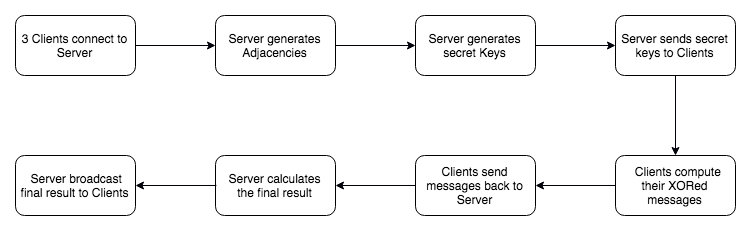
\includegraphics[width=1\textwidth]{Images/Implementation/protocolExecuted.png}
    \caption{Main steps of protocol successfully executed}
    \label{fig:protocolExecuted}
\end{figure}

Beside the main steps described and presented in figure \ref{fig:protocolExecuted}, there are more underlying \lstinline{socket.io} events communicated in order to update the graphical user interface of the user and provide explicate content about each stage of the protocol.

\begin{figure}[H]
    \centering
    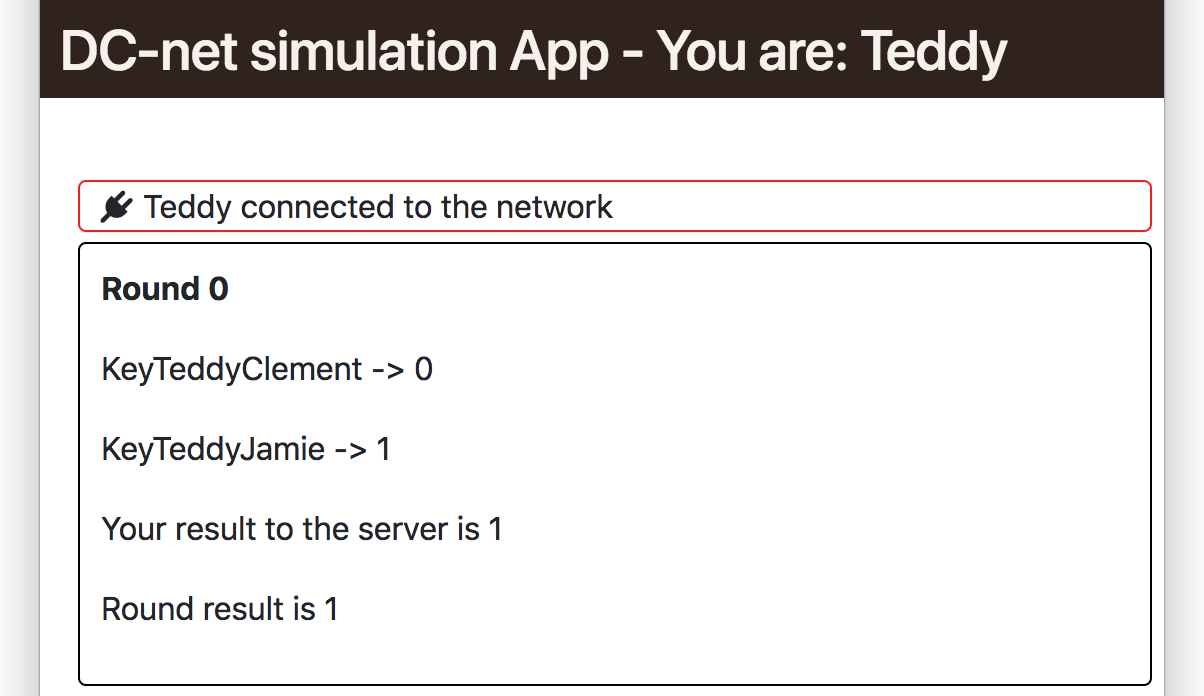
\includegraphics[width=0.5\textwidth]{Images/Implementation/singleRoundExecuted.png}
    \caption{UI at the completion of one successful round.}
    \label{fig:singleRoundExecuted}
\end{figure}


\subsection{HTTPS only on deployed application}
The solution proposed to exchange secret keys securely is to employ secure HTTP protocol, i.e. HTTPS, to connect with the web sever. This ensure that keys cannot be seen by an eavesdropped. In fact, this actually seals not only the key sharing phase but whole of the communication with encryption.

\begin{lstlisting}
    // function credit to https://stackoverflow.com/a/31144924/3245486
    function requireHTTPS(req, res, next) {
        // The 'x-forwarded-proto' check is for Heroku
        if (!req.secure && req.get('x-forwarded-proto') !== 'https' && process.env.NODE_ENV !== "development") {
            return res.redirect('https://' + req.get('host') + req.url);
        }
        // allow next incoming requests
        next();
    }
    
    // enforce https on production
    if(process.env.NODE_ENV === 'production') {
        app.use(requireHTTPS);
    }
\end{lstlisting}


\section{Advanced Implemented System}
This section presents the final implemented system, which includes all the advanced requirements. The codebase is more complex and the features presented are the main additions to the platform presented before.


\subsection{Arbitrary number of participants} \label{sec:arbitraryPartipantN}
To execute the protocol with an arbitrary number of participants is enough to accept all incoming connections, instead of throwing an error when a fourth participant tries to connect, as shown in section \ref{sec:triggerProtocol}. The real challenge of supporting an arbitrary number of participants is to handle connections and disconnection throughout the execution of the protocol. This problem was not present with only three clients, as this was the both the minimum and maximum number of participants in the network, and any variation of participants would simply stop the execution of the protocol. \newline

To support incoming connections during the protocol execution, a participant is added to a list of pending participants, instead of joining the simulation immediately. To improve the user experience, the waiting participants is also informed of such event with a clear message.

\begin{lstlisting}
    // if simulation started make participant wait.
    if(simulationStarted) {
        pendingParticipants = [...pendingParticipants, newParticipant];
        // inform user that he is waiting 
        unicastEvent(newParticipant.id, 'display-waiting-message');
    } else {
        // allow user to join the simulation straight away.
    }
\end{lstlisting}

Only at the end of the protocol pending participants can then join the simulation.

\begin{lstlisting}
    function addPendingParticipantsToSimulation() {
        // join simulation by being added to participants array
        participants = [...participants, ...pendingParticipants];
        pendingParticipants.forEach(function (pendingParticipant) {
            unicastEvent(pendingParticipant.id, 'hide-waiting-message');
        });
        pendingParticipants.length = 0;
    }
\end{lstlisting} 


To support disconnections of participants during the protocol execution instead, the simulator immediately removes the participant from the simulation. His neighbouring clients update their key values so as to preserve the correctness of the protocol execution. For the sake of brevity the code of this functionality is omitted from the main report, but it can be found in the appendix \ref{appendix:code}, specifically in the \lstinline{chat-server.js} file.

\subsubsection{Browser Connections Limit}
It is important to note that modern browsers allow a limited number of persistent connections per domain. The average number of connections allowed is 4 to 6 \cite{Souders}. Therefore, it turns out that trying to test this application from a single machine using Chrome browser, it is only possible to open 5 browser tabs that connect to the DC-Net server. Using multiple browsers allows to grow this number for testing purposes from the same computer.


\subsection{Voting, Length-Calculation, Communication Round}
The final simulator includes three types of rounds as first presented in section \ref{sec:advancedReq}. Each type of round has its own dedicated functions to start the round, to generate and share secret keys, handle results on the server and so on. This is due to the fact that despite being similar, each of the round types presents some variations.

The voting round uses 1-bit keys and it tries to simply determine who will send a message. This round type is repeated until someone decides to send a message and wins the voting round.

The length-calculation rounds allows the message sender to provide a sentence, in the time span of 10 seconds. After this time, all participants browsers, including the non sender's one, will automatically dispatch the response to the server. The time span is fixed for all participants, to avoid a scenario in which the message sender takes a long time to write a message. In such case, the sender would be reveal by simply looking at the which message was received last by the server. Due to the limited time frame, the message sender has 3 attempts to provide the sentence. In addition, the key will be a secure random value in between 100 and 999. I chose this range to avoid a scenario in which all the secret keys are very short numbers to be XORed with the message length. If this latter value would be considerably longer than the keys themselves, untraceability of the sender could be compromised by looking at which is the greater response sent to the server. 

Lastly, there is a number of communication rounds, one for each letter of the sentence provided. These rounds happens with a short delay between each other, and at the end the aggregate message received will be shown. Communication round use 8-bit keys, useful to hide the corresponding number of a EASCII character, as explained in the next section. In order to generate n keys, I employed the \lstinline{crypto} JavaScript in-built module to generate an array of cryptographically secure pseudo-random numbers.

\begin{lstlisting}
    function secureRandomKeyArrayOfLength(n) {
      // 8 bits goes from 0 to 255
      let pseudoRandom = new Uint8Array(n);
      let bytes = crypto.randomBytes(n);
      pseudoRandom.set(bytes);
      return Array.from(pseudoRandom);
    }
\end{lstlisting}


\subsection{EASCII encoding conversion}
As one of the main contributions, I proposed to interpret a the value of a round message as a EASCII code. Thus, the sentence provided by the message sender (figure \ref{fig:exampleMessage}) will be a series of EASCII characters (figure \ref{}), and at each communication round the corresponding EASCII code of the nth letter will be XORed with the two secret keys that the sender participant possess.

\begin{figure}[H]
    \centering
    \fbox{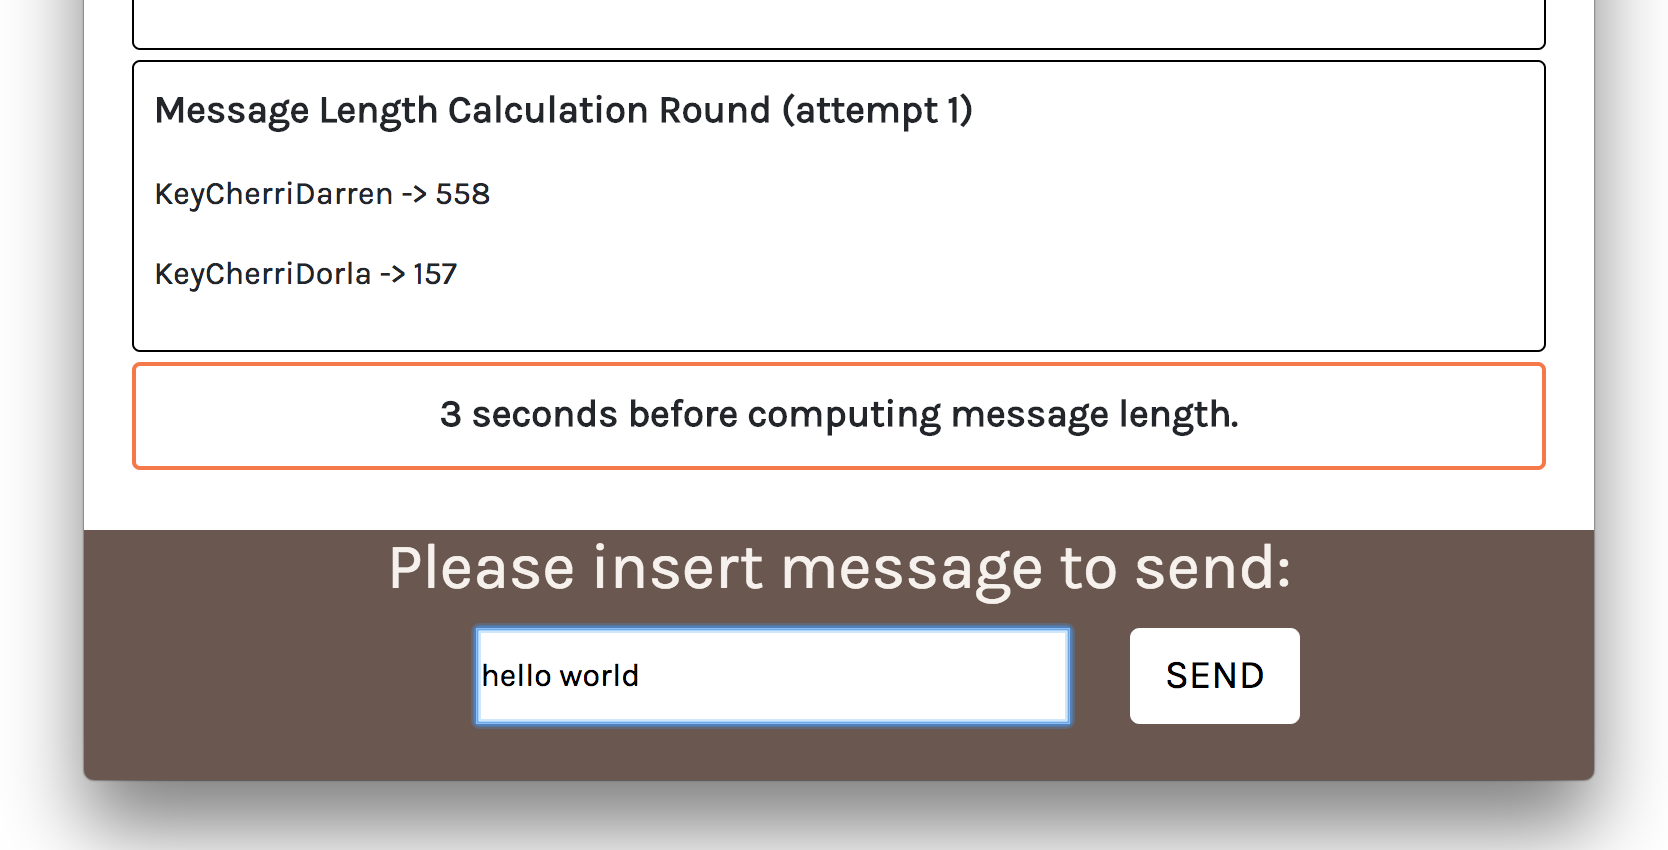
\includegraphics[width=0.6\textwidth]{Images/Implementation/exampleMessage.png}}
    \caption{Example of sentence provided by message sender }
    \label{fig:exampleMessage}
\end{figure}


\begin{figure}[H]
    \centering
    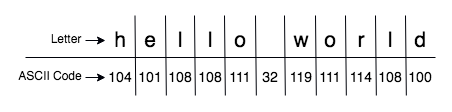
\includegraphics[width=0.70\textwidth]{Images/Implementation/messageInASCII.png}
    \caption{Interpretation of message in EASCII encoding}
    \label{fig:exampleInASCII}
\end{figure}

For example, in the first communication round of the message shown in figure \ref{fig:exampleMessage}, if the two secret keys of the message sender are 207 and 91. The round message sent to the server would be $M = 207 \oplus 91 \oplus 104 = 252$.

The conversion from a character to its corresponding EASCII code and vice versa is achieves in JavaScript with simple in-built functions of the String object: 
\begin{lstlisting}
    // obtain EASCII code number of a letter from a string called 'sentence'
    var EASCIIcode = sentence.charCodeAt(letterIndex);

    // obtain a letter from a give EASCII code
    var letter = String.fromCharCode(EASCIIcode);
\end{lstlisting}



\subsection{Collision Detection}
Detecting collisions is important to ensure that only one participant can send a message per round. In order to do so, the secret keys are generated and stored on the server and then sent to the two participants of a given adjacency. 

\begin{lstlisting}
    // create key names based on the name of the participants in the adjacency
    var keyName1 = 
        'Key' + adjacency.participant1.name + adjacency.participant2.name;
    var keyName2 = 
        'Key' + adjacency.participant2.name + adjacency.participant1.name;
    // store keys on the server
    adjacency.participant1.keys = 
        [...adjacency.participant1.keys, {keyName: keyName1, keyValue}];
    adjacency.participant2.keys = 
        [...adjacency.participant2.keys, {keyName: keyName2, keyValue}];
    // send keys to clients
    unicastEvent(adjacency.participant1.id, 'round-key-generated', [keyName1, keyValue]);
    unicastEvent(adjacency.participant2.id, 'round-key-generated', [keyName2, keyValue]);
\end{lstlisting}


Then, when a participants sends his round response to the server, the handler function that manages the received responses contains some conditional statements to deal with the different cases. The server computes the expected message, which is the result of XORing only the secret keys when a participants does not attempt to send a value. If the received message is the same as the expected message, then it is simply accepted. However, if the message is different from the XOR of the two secret keys, it means that the client is trying to send a message. Therefore, if someone has already sent a message in this round, the attempt to send a message is rejected, otherwise it is accepted.

\begin{lstlisting}
    function(participantMessage) {
        // finding sender with the socket.id of the incoming event
        const sender = findParticipantbyId(participants, socket.id);
        const expectedMessage = sender.participantExpectedXORValue();
        if(participantMessage === expectedMessage) {
            sender.roundMessage = participantMessage;
        } else {
            if (rounds[currentRoundIndex].didSomeoneSendMessage) {
                sender.roundMessage = expectedMessage;
                /* add participants to list of rejected participants. These will be notified of the rejection when all the round responses are received on the sever. */
                rejectedParticipants = [...rejectedParticipants, sender];
            } else {
                sender.roundMessage = participantMessage;
                rounds[currentRoundIndex].didSomeoneSendMessage = true;
                // make this sender, the message sender for this round
                messageSender = sender;
            }
        }
    }
\end{lstlisting}

This mechanism is employed in necessary only in the \lstinline{handleVotingRoundParticipantResponse} round. After the the winner of the voting round is established, other non-sender clients are not given the possibility to send their specific message back, and the XOR of their two secret keys is automatically sent back to the server. Therefore, the collision detection mechanism is not strictly necessary for the other type of rounds, however, it is still present in the handlers so as to address the case in which a user would try to change values manually inside the storage of the browser.


\subsection{Helper hover notes}
Since the protocol may be a bit confusing for a new learner, short helper messages have been included in the application (figure \ref{fig:helperMessageExample}). These can be enabled/disabled from the controls dropdown provided in the right corner of the simulator (figure \ref{fig:controlsDropdown}). In addition, since the messages are displayed by hovering on the relevant question mark icon and the simulation has an automatic scroll, the user can also disable the scrolling functionality.

\begin{figure}[H]
    \centering
    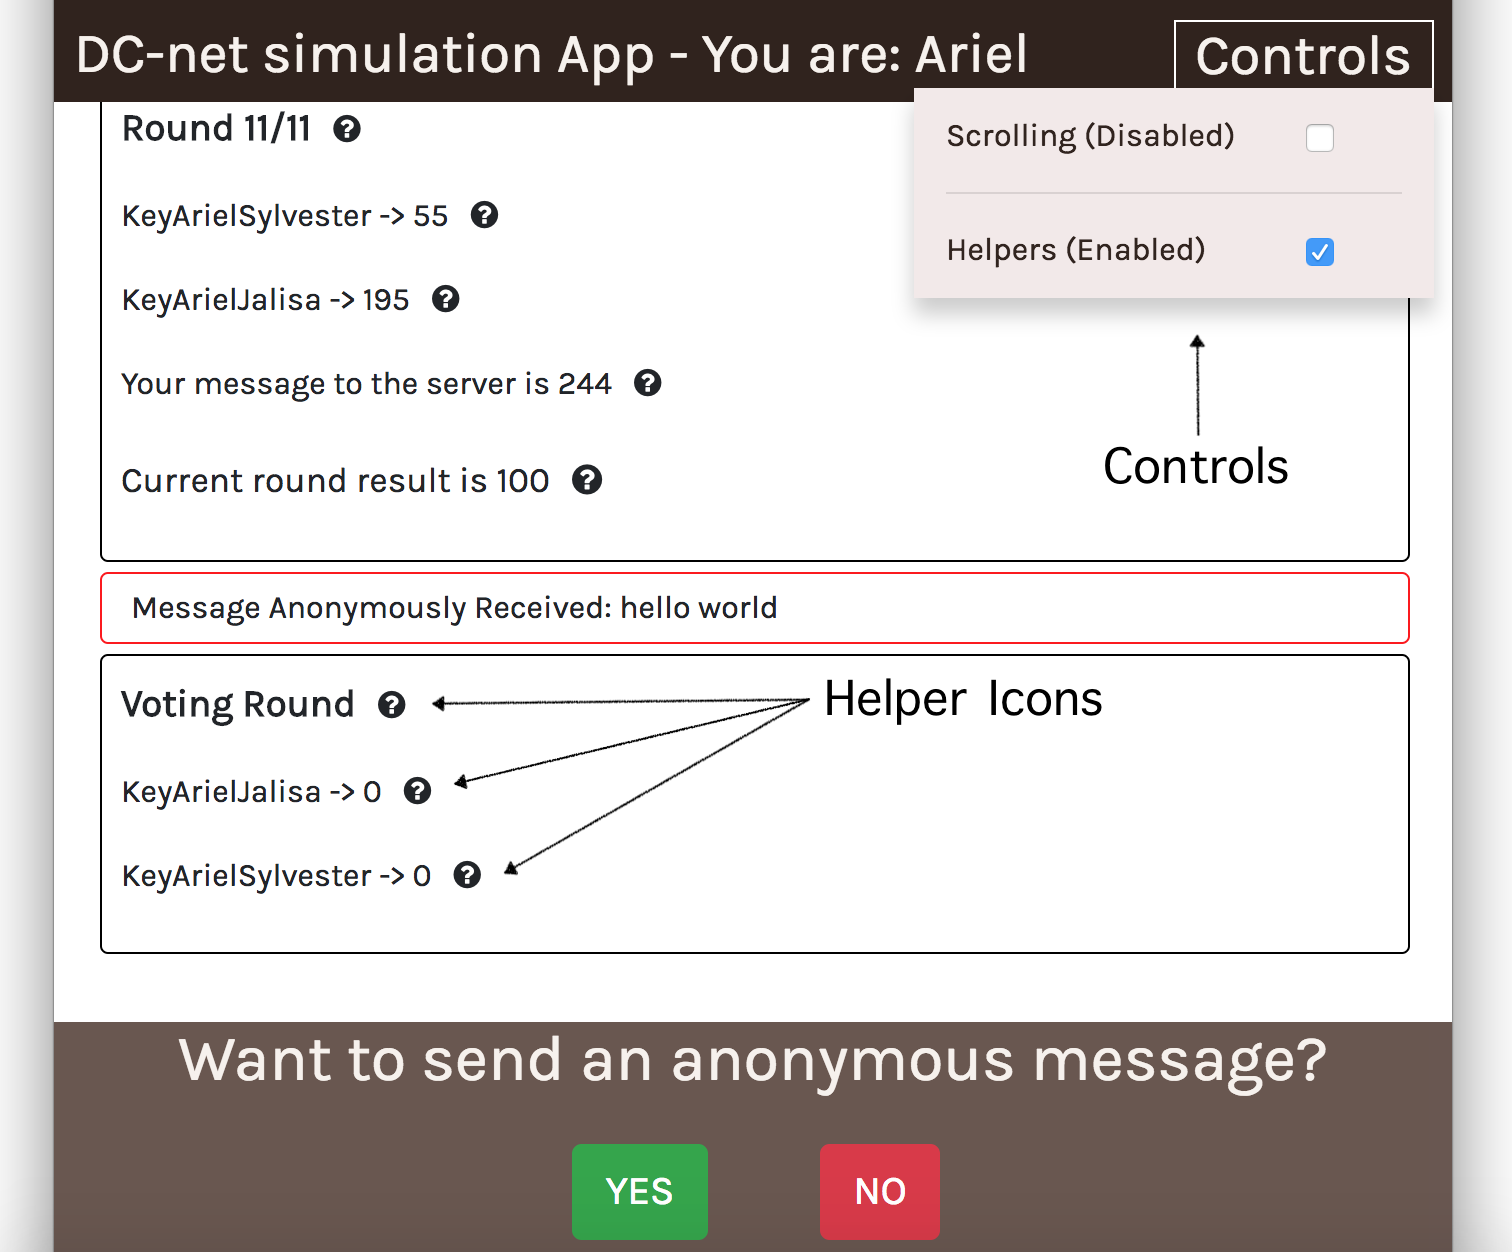
\includegraphics[width=0.70\textwidth]{Images/Implementation/controlsDropdown.png}
    \caption{Dropdown controls to show helper message icons}
    \label{fig:controlsDropdown}
\end{figure}

\begin{figure}[H]
    \centering
    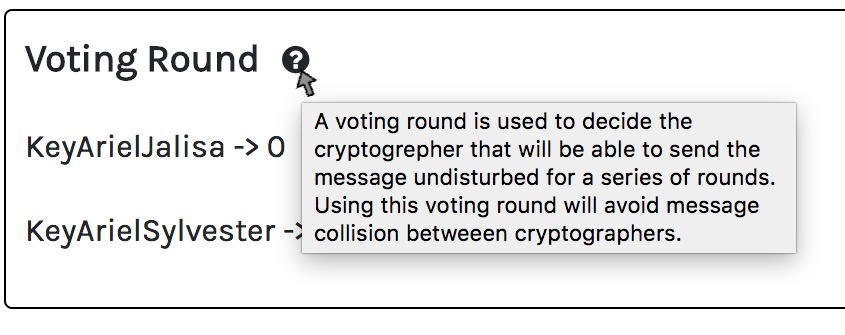
\includegraphics[width=0.50\textwidth]{Images/Implementation/helperMessageExample.png}
    \caption{Example of helper message on hover}
    \label{fig:helperMessageExample}
\end{figure}




\section{Unit Testing}
Unit testing is the execution of tests on small parts of the codebase, usually one function at a time. This happens by running a given function with some chosen input and comparing the expected output with the actual output. 

Not only unit testing has the main purpose of checking the correct execution of the logic of the application, but it also helps to break down the codebase into separate functions, each one with its specific purpose, since it would otherwise be difficult to test them.

The framework Mocha with help of Chai assertion library (see section \ref{sec:testingFrameworks}) were used. The tests are included in the source code in \lstinline{./test/test.js}.

\section{Implementation challenges}
Although the architecture of the simulator was not particularly complex, I faced a number of challenges throughout the implementation phase that arose to ensure correctness at all times and preserve constant untraceability. 

\subsection{Protocol execution in real time and distributed across nodes}
The event-based library \lstinline{socket.io} was chosen for its high-level API and simplicity of use. However, it was important to firstly experiment with this library in order to understand how to integrate the real-time communication with the protocol logic. The main challenge was to discern the different components that should be executed on the client's browser from the parts to be performed on the server.

\subsection{Ensure protocol correctness}
As mentioned in section \ref{sec:arbitraryPartipantN}, there was a number of issues deriving from allowing an arbitrary number of connection to the server. Dealing with connecting and disconnecting participants during the protocol execution was a problem not though of beforehand that instead arose one of the other. Such as, if the message sender disconnects throughout the communication rounds, abort the communication. However, if a participant wins the voting round before all clients have provided their response, and this disconnects, then instead simply allow remaining clients to win the round. 

\subsection{Retain sync between front-end and back-end state}
Another important part to reason correctly about the protocol execution from the programmer standpoint was to mimic the state of the server on clients correctly and vice versa. Thus, if there was an update on any of the clients it was important to communicate it, whenever this does not compromise untraceability, to the server so as to be able to have at least a partial synchronization of information between the different principals, which is useful to make safe assumption about which data is available at each stage of the protocol execution.


\section{Mapping Theoretical Concepts to Implementation}
This section has the purpose to recap the correlation between the initial concepts of the analogy and formal protocol with the implemented software. \newline

The exposition of the Dining Cryptographers first started with a number of cryptographers dining at a restaurant. These represented nodes of a graph that in the implemented simulation are represented by users connecting to the DC-Net server through their browser. \newline

The purpose of executing the protocol at the dinner was to find out if someone paid for the dinner or if their employer did so. The actual protocol execution has the purpose to see if someone sent a message, and the final broadcasted result is the message itself. Therefore, paying the dinner corresponds to a node sending a message. In the scenario that uses 1-bit keys, the action of sending a message is also referred to as flipping one's message. In the software implemented, sending a message corresponds to a participant attempting to XOR a chosen value with his two secret keys before sending the result of this operation to the server. \newline

The coin flipped behind a menu is the key-exchange procedure that needs to take place securely, not only in respect to the participants that are not part of the given adjacency but in respect to every possible adversary that on the network. In the simulation, the central DC-Net service generates all keys with a cryptographically secure pseudo-random number generator and delivers them to the clients via \lstinline{https} protocol. \newline

